% Copyright 2007 by Till Tantau
%
% This file may be distributed and/or modified
%
% 1. under the LaTeX Project Public License and/or
% 2. under the GNU Public License.
%
% See the file doc/licenses/LICENSE for more details.



\documentclass{beamer}

% Setup appearance:

%\usecolortheme[RGB={0,0,0}]{structure} 
%\definecolor{Unidblue}{RGB}{255,0,0}
%\definecolor{dgreen}{rgb}{0.,0.6,0.}
%\setbeamercolor{title}{fg=Unidblue}
%\usetheme{boxes}
%%\usefonttheme[]{default}
%\setbeamerfont*{frametitle}{size=\normalsize}
%%\setbeamertemplate{navigation symbols}{}
%\setbeamertemplate{footline}[page number]
\definecolor{dblue}{RGB}{83,121,170}
%
%\newenvironment{wideitemize}{\itemize\addtolength{\itemsep}{10pt}}{\enditemize}
%
%\setbeamercolor{alerted text}{fg=gray,bg=}
%\setbeamercolor{normal text}{fg=black,bg=}
%\usebeamercolor{normal text}


\newcommand\numbered{\setbeamertemplate{footline}{%
\raisebox{5pt}{\makebox[\paperwidth]{%
\hfill\makebox[10pt]{%
\scriptsize\insertframenumber}}}}}
\newcommand\unnumbered{\setbeamertemplate{footline}{}}

% Standard packages
\usepackage[english]{babel}
\usepackage[latin1]{inputenc}
\usepackage{times}
\usepackage{xcolor}
\usepackage[T1]{fontenc}
\usepackage{bbm}
\usepackage{subfigure}
\usepackage{pgf,pgfarrows,pgfnodes}
\usepackage{tikz}
\usetikzlibrary{arrows,shapes}

\usetheme{Boadilla}
\setbeamertemplate{itemize items}[default]
\setbeamertemplate{enumerate items}[default]

%\AtBeginSection[] %GOOD CODE! Will add an outline slide before each section
%{
%   \begin{frame}
%       \frametitle{Outline}
%       \tableofcontents[currentsection]
%   \end{frame}
%}

% Setup TikZ

% Author, Title, etc.

\title{\textcolor{black} {Simulation approaches for assessing the impacts on equity in a region  due to earthquakes}}
%Network risk mitigation by simulating failures in lifeline networks}}
% Simulating failures in lifeline networks from natural disasters enables risk mitigation with a system performance perspective

\author{{\textcolor{dblue} {Mahalia Miller and Jack Baker \\ Stanford University}}}


\institute[Stanford University]
  
\date[defense 2013]
{ \textcolor{dblue} {SRA,  December 10, 2013}}
%mission is to support the global risk and disaster management needs of today, using the technologies of tomorrow
% The main document
\begin{document}

\numbered
\begin{frame}
  \titlepage
\end{frame}


%\numbered
%  \begin{frame}[t]{What's the likelihood of travel disruptions due to a natural disaster?}
%  \centerline{ \includegraphics[height=0.75\textheight]{Visuals/1/zoomedtobay2.pdf}}
%  \end{frame}
%  
  
  \begin{frame}[t]{How might extensive earthquake damage to US-101 disrupt the daily commute of people in Palo Alto versus San Francisco?}
  \centerline{ 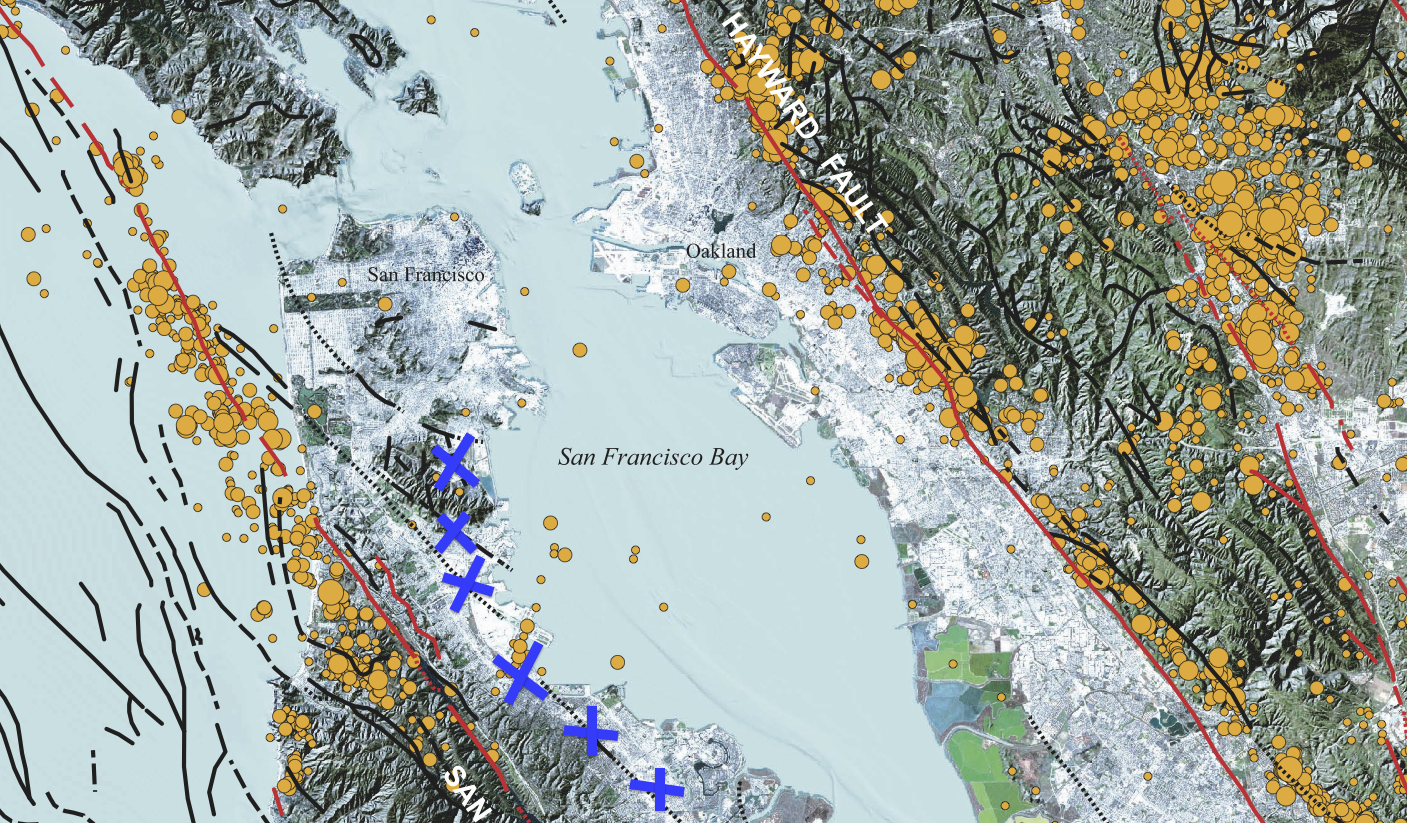
\includegraphics[height=0.75\textheight]{zoomedToSF_no101.png}}
        \tiny Image source: Modified from United States Geological Survey (USGS)
  \end{frame}
  
%\begin{frame}
%       \frametitle{Outline}
%       \tableofcontents %works with multiple sections
%   \end{frame}

   %%%%%%%%%%%%%%%%%%%%%%%%%%%%%%%%%%%%%%%%%%%%%%%%%%%%
 
    \section{Limitations in existing methods} 
    
            \numbered
            \begin{frame}[t]{Challenges}
              \vspace{5mm}

            The research problem is to assess the risk of natural disasters to lifeline networks 
          \vspace{2mm}

        \begin{itemize}
        \item at a large scale,
          \vspace{2mm}

        \item     in a risk-consistent probabilistic approach and
          \vspace{2mm}

        \item examining the network impacts not only globally (region-wide) but also for individual communities and socio-economic groups
        \end{itemize}
%            a.) large scale, b.) in a risk-consistent probabilistic approach, and c.) examining the network impacts not only globally (region-wide) but also for individual communities and socio-economic groups.
            \end{frame}
    
    %%%%%%%%%%%%%%%%%%%%%%%%%%%%%%%%%%%%%%%%%%%%%
    
  \numbered
  \begin{frame}[t]{...}
  \end{frame}
  
    \numbered
  \begin{frame}[t]{Summary}
  \vspace{5mm}
  Today I have shown a method for assessing the impacts of earthquakes on equity. Results from a case study of the San Francisco Bay Area suggest:
    \vspace{5mm}
     \begin{enumerate}
      \item Some geographic regions are at higher risk than others, particularly where there is limited public transit and/or limited redundancies in the roads      
      \vspace{5mm}
    \item Wealthier households may be at higher risk of losses in accessibility
           \vspace{5mm}
    \item Prioritizing bridge retrofits by highest risk of collapse is different than prioritizing by impact on accessibility 
          \vspace{5mm}
    \end{enumerate}
  \end{frame}

  \numbered
  \begin{frame}[t]{...}
  \end{frame}
    
\end{document}


